% !TEX root = ci223-project-plan.tex
% !TEX program = lualatex

% Template for MSc final reports
% ESE Department - Imperial College London
%
% INSTRUCTIONS
% (1) Compile using LuaLatex (it is the successor of pdflatex). To check this on Overleaf, click on the Menu on the top left.
% (2) Complete the SETUP below
% (3) Students of Imperial College can claim a free premium Overleaf account, see https://www.imperial.ac.uk/admin-services/ict/self-service/computers-printing/devices-and-software/get-software/get-software-for-students/overleaf/ 
% Claim the free premium account because as your report becomes more and more complex you may reach the timeout limit of the free account.

%%%%%%%%%%%%%%%%%%%%%%%%%%%%%%%%%%%%%%%
% DO NOT MODIFY FROM HERE ...
\documentclass[11pt]{ic_ese_thesis}

\usepackage[style=ieee,backend=biber,hyperref=auto]{biblatex}
\addbibresource{references.bib}
% ... TO HERE
%%%%%%%%%%%%%%%%%%%%%%%%%%%%%%%%%%%%%%%


%%%%%%%%%%%%%%%% SETUP %%%%%%%%%%%%%%%%
%%%%%%%%%%%%%%%%%%%%%%%%%%%%%%%%%%%%%%%
% EDIT THE FOLLOWING INFORMATION WITH YOUR DATA
% COMPLETE PART A
% IF YOU ARE DOING A MENG/BENG COMPLETE ALSO PART B
% IF YOU ARE DOING AN MSC IGNORE PART B
% LINES STARTING WITH % ARE COMMENTS. UNCOMMENT JUST ONE OF A SET OF OPTIONS
% MAKE SURE YOU CHECK AND UPDATE ALL INFORMATION, INCLUDING SUBMITYEAR

%%%%%%%%%%% PART A %%%%%%%%%%%

\degree{MSc}

\title{Innovative Approaches to Asset Prediction: Combining Deep Learning with Financial Modelling}
\subtitle{Final Report} % use \subtitle{} to remove the subtitle
\author{C. Ioannidis}
\cid{02533490}
\supervisor{Prof. Pasquale Della Corte \\[1mm] Prof. Walter Distaso \\[1mm] Dr Lluis Guasch} %UK: Dr no dot, prof has dot
\submityear{2024}

\course{Applied Computational Science and Engineering}



% Do you want a list of figures?
% Do you want a list of tables?
% Do you want an acknowledgement page?
% Do you want a list of acronyms?
\setboolean{list_of_figures}{false} % false or true - Default is true
\setboolean{list_of_tables}{false} % false or true - Default is false
\setboolean{acknowledgement}{false} % false or true - Default is true
\setboolean{acronyms}{false} % false or true - Default is true

\setboolean{edge_labels}{true} % default for MSc


\setboolean{double_spacing}{true} %Default is true. If you want to change this, ask your supervisor if they are OK with singlespacing.

%%%%%%%%%%% PART B %%%%%%%%%%%
% ONLY FOR MENG/BENG. MSC IGNORE THIS
% THESE ADDITIONAL SETTINGS HAVE BEEN ASKED BY THE MEng COMMITTEE BUT NOT BY THE MSC COMMITTEE
% Is this an interim report or final thesis?
\setboolean{final_thesis}{true} % true for final Thesis / false for interim report
\secondmarker{} %If you do not know who your second marker is, use \secondmarker{}

%%%%%%%%%%%%% END SETUP %%%%%%%%%%%%%%%
%%%%%%%%%%%%%%%%%%%%%%%%%%%%%%%%%%%%%%%


% ADDITIONAL PACKAGES
% You can add your packages below. Note that the following packages are already loaded: pgfcore, geometry, bookmark, graphicx, setspace, kantlipsum, fontspec, polygrossia (default English), minitoc, silence, background, xpatch, tikzpagenodes, totcount, fancyhdr, titlesec and the tikz libraries calc, shapes.symbols and shapes.misc  

%Examples
\usepackage{amsmath}
\usepackage{amsfonts}
%...

\begin{document}

\thesisspacing

\preamble % Do not change - required

% EDIT THE CONTENT OF THE FILES
% Abstract.tex
% OrigSta_Copyright.tex
% Acknowledgement.tex
% You can find them under the folder
% "chapters" on the left column

% ADD AS MANY CHAPTERS AS NEEDED
% BY CREATING .TEX FILES IN THE FOLDER chapters
% AND ADDING \input{namechapter.tex} BELOW
\thesisspacing
\doublespacing % Do not change - required

\chapter{Introduction}
\label{ch1}

%%%%%%%%%%%%%%%%%%%%%%%%%%%%%%%%%%%%%%%
% IMPORTANT
\begin{spacing}{1} %THESE FOUR
\minitoc % LINES MUST APPEAR IN
\end{spacing} % EVERY
\thesisspacing % CHAPTER
% COPY THEM IN ANY NEW CHAPTER
%%%%%%%%%%%%%%%%%%%%%%%%%%%%%%%%%%%%%%%

\section{Introduction}
%%%%%%%%%%%%%%%%%%%%%%%%%%%%%%%%%%%%%%%
\thesisspacing % CHAPTER
% COPY THEM IN ANY NEW CHAPTER
%%%%%%%%%%%%%%%%%%%%%%%%%%%%%%%%%%%%%%%

The prediction of financial markets has undergone significant evolution in recent years, driven largely by advancements in machine learning techniques. This study explores the use of Convolutional Neural Networks (CNNs) as advanced predictive models for analyzing time-series data across various asset classes. The primary objective of this research is to enhance the accuracy of financial market predictions by employing CNN architectures capable of capturing the complex patterns inherent in financial data. This project involves a comprehensive approach, beginning with the collection and preprocessing of extensive time-series datasets, followed by the development and iterative refinement of CNN-based models that address the unique challenges posed by financial market forecasting.

\section{Background and Motivation}
%%%%%%%%%%%%%%%%%%%%%%%%%%%%%%%%%%%%%%%
\thesisspacing % CHAPTER
% COPY THEM IN ANY NEW CHAPTER
%%%%%%%%%%%%%%%%%%%%%%%%%%%%%%%%%%%%%%%

Traditional methods for predicting financial markets, such as the Auto Regressive Integrated Moving Average (ARIMA) model, have been widely applied but often struggle to capture the nonlinear and intricate dynamics of financial data. The advent of machine learning, and specifically CNNs, has introduced more sophisticated techniques capable of addressing these limitations. Recent research has demonstrated the efficacy of CNNs in financial market prediction by transforming time-series data into visual formats that can better capture underlying patterns.

For instance, Kusuma et al. (2019) utilized CNNs to analyze historical stock data converted into candlestick chart images, achieving high prediction accuracy for stock markets in Taiwan and Indonesia \cite{kusuma2019using}. Sezer and Ozbayoglu (2019) further advanced this approach by transforming time-series stock data into 2-D bar chart images and applying CNNs to identify trading signals, demonstrating superior performance to traditional methods, especially during bearish market conditions \cite{sezer2019financial}. Zeng et al. (2021) expanded on these concepts by introducing a video prediction model for economic time series that leveraged CNNs' ability to detect spatial patterns in image sequences, outperforming traditional techniques like ARIMA and Prophet \cite{zeng2021deep}. Jiang (2023) also employed CNNs with OHLC (Open, High, Low, Close) charts to forecast stock returns, highlighting the model's capacity to recognize intricate patterns and adapt across different geographical and temporal scales \cite{jiang2023reimagining}. Collectively, these studies underscore the potential of CNNs to significantly improve asset price prediction accuracy, offering a marked advantage over traditional forecasting methods.


\section{Research Objectives}
%%%%%%%%%%%%%%%%%%%%%%%%%%%%%%%%%%%%%%%
\thesisspacing % CHAPTER
% COPY THEM IN ANY NEW CHAPTER
%%%%%%%%%%%%%%%%%%%%%%%%%%%%%%%%%%%%%%%

The primary goal of this research is to enhance the predictive capabilities of financial market models through the development and refinement of CNN architectures. By focusing on the analysis of time-series data, this study aims to uncover complex patterns that drive market behavior, thus facilitating more accurate and reliable predictions. Achieving higher predictive accuracy is expected to support more effective risk management strategies, particularly in volatile market environments. Additionally, this research seeks to provide insights that can assist investors and financial analysts in making more informed decisions regarding investment strategies, thereby contributing valuable knowledge to the field of financial analytics. The overarching aim is to advance the adoption of more sophisticated machine learning techniques in financial forecasting, promoting a deeper understanding of global market dynamics.



\section{Methodology Overview}
%%%%%%%%%%%%%%%%%%%%%%%%%%%%%%%%%%%%%%%
\thesisspacing % CHAPTER
% COPY THEM IN ANY NEW CHAPTER
%%%%%%%%%%%%%%%%%%%%%%%%%%%%%%%%%%%%%%%

The methodological approach of this study encompasses several stages. Initially, extensive time-series data will be collected and preprocessed to ensure it is suitable for deep learning applications. The data will then be transformed into image formats, such as candlestick charts, to facilitate the training of CNN models. Following data preparation, various CNN architectures will be developed and iteratively refined to optimize their predictive performance. The models will be trained using historical market data to learn patterns and trends that may inform future market movements.

In the final stages of the project, the developed models will be tested within simulated environments to assess their accuracy and practical applicability in real-world scenarios. This evaluation will be conducted through rigorous backtesting and benchmarking against standard market indices, such as the S\&P 500, to measure their performance relative to traditional investment strategies.

\section{Expected Contributions}
%%%%%%%%%%%%%%%%%%%%%%%%%%%%%%%%%%%%%%%
\thesisspacing % CHAPTER
% COPY THEM IN ANY NEW CHAPTER
%%%%%%%%%%%%%%%%%%%%%%%%%%%%%%%%%%%%%%%

The anticipated outcomes of this research are expected to provide significant insights into market dynamics, thereby enhancing the decision-making processes in financial investments. By demonstrating the practical utility of CNNs in financial forecasting, this study aims to bridge the gap between theoretical advancements and their real-world applications in financial markets. The findings are expected to contribute substantially to the field of financial analytics, promoting the integration of advanced machine learning techniques into market prediction and portfolio management strategies. This research represents a meaningful contribution to the ongoing discourse on the application of deep learning in financial markets, with implications for both academic research and practical investment decision-making.


\thesisspacing
\doublespacing % Do not change - required

\chapter{Methodology}
\label{ch2}

%%%%%%%%%%%%%%%%%%%%%%%%%%%%%%%%%%%%%%%
% IMPORTANT
\begin{spacing}{1} %THESE FOUR
\minitoc % LINES MUST APPEAR IN
\end{spacing} % EVERY
\thesisspacing % CHAPTER
% COPY THEM IN ANY NEW CHAPTER
%%%%%%%%%%%%%%%%%%%%%%%%%%%%%%%%%%%%%%%

% \section{Training}
% %%%%%%%%%%%%%%%%%%%%%%%%%%%%%%%%%%%%%%%
\thesisspacing % CHAPTER
% COPY THEM IN ANY NEW CHAPTER
%%%%%%%%%%%%%%%%%%%%%%%%%%%%%%%%%%%%%%%

\subsection{Data Preprocessing and Integration}

The preprocessing phase was a critical step in preparing the data for effective training of the Convolutional Neural Network (CNN) model. Given the nature of financial time-series data and the need to convert it into formats suitable for deep learning, a rigorous and systematic approach was adopted.

Initially, the data underwent a comprehensive cleaning process to address inconsistencies, missing values, and outliers. As the data was sourced from multiple repositories—namely CRSP, Kaggle, and Yahoo! Finance—standardization across datasets was paramount. Missing values were handled using techniques such as forward and backward filling to maintain the temporal continuity of the data, while outliers were identified and removed using statistical methods like Z-score analysis and interquartile range (IQR) filtering. This step was essential to ensure that the data fed into the CNN models was both reliable and representative of typical market behaviors.

Following the cleaning process, normalization was applied to standardize the range of the OHLC (Open, High, Low, Close) data. Normalization is crucial in neural network models to ensure that all input features contribute equally to the learning process. This typically involved scaling the OHLC data to a range between 0 and 1, which helps in achieving faster convergence during the training phase and avoids biases that could arise from differing magnitudes in raw data values.

A significant aspect of the preprocessing phase was the transformation of the normalized OHLC data into 64x64 pixel images, specifically candlestick charts, which serve as the primary input format for the CNN models. The transformation process involved converting sequential OHLC data points into a series of candlestick charts, capturing the temporal dynamics and price movements over fixed intervals. These images were then stored in .npy files, an efficient format for handling large-scale image datasets within NumPy arrays, enabling streamlined data loading and manipulation during the training phase.

This approach of converting OHLC time-series data into visual representations leverages the ability of CNNs to recognize complex spatial patterns, which are indicative of underlying market trends and behaviors. By using a visual representation, the CNN model is better positioned to learn from patterns in the data that are not easily captured through traditional numerical methods, thus enhancing the robustness and accuracy of the predictive model.

\subsection{Model Development and Training}

The development and training of the CNN model were meticulously structured to explore various architectural configurations aimed at maximizing predictive accuracy while minimizing overfitting. The chosen architecture treated the model as a classifier, designed to predict market direction based on the input images derived from OHLC data.

The initial phase of model development involved experimentation with multiple CNN architectures to identify the most effective structure for financial market prediction. This experimentation included testing various combinations of convolutional layers, pooling layers, and activation functions. Key architectural features such as dropout layers were integrated to reduce overfitting by randomly deactivating a subset of neurons during each training iteration. This technique helps to generalize the model, ensuring it does not overly fit the training data at the expense of performance on unseen data.

Residual blocks were also employed to enhance the model's depth and ability to capture complex features. Residual connections facilitate the training of deep networks by allowing gradients to flow more effectively through multiple layers, preventing the vanishing gradient problem commonly encountered in deep learning. This capability is particularly valuable in financial modeling, where deep architectures can uncover complex, non-linear relationships inherent in market data.

In addition to standard CNN layers, the model architecture incorporated Long Short-Term Memory (LSTM) layers to capture sequential dependencies in the time-series data. LSTMs, a type of recurrent neural network (RNN), are well-suited for handling sequences and can retain information across time steps, making them ideal for capturing the temporal dependencies crucial in financial forecasting.

The training dataset, encompassing randomly selected stocks from the U.S. market from the 1990s until 2017, was deliberately chosen to ensure that the model trained on data entirely unrelated to the backtesting period (June 2019 to June 2024). This strategic choice was aimed at preventing any data leakage between the training and testing phases, thereby enhancing the model's generalizability and ensuring that performance metrics reflect true predictive power rather than overfitting to historical data.

The training process involved optimizing the model's parameters through iterative tuning of hyperparameters such as learning rates, batch sizes, and epochs. Optimization algorithms, including Adam and RMSprop, were explored to identify the most effective approach for minimizing the loss function and achieving stable convergence. The model's performance was continuously evaluated using classification metrics such as accuracy, precision, recall, and F1 score, which provided an outline of which configurations were likely to perform best during the subsequent backtesting phase.

By rigorously testing and refining these CNN architectures, the study aimed to identify the model configuration that most effectively captures the complex patterns in financial data, providing a robust tool for predicting market movements and contributing valuable insights to the field of financial analytics.

% \section{Evaluating}
% %%%%%%%%%%%%%%%%%%%%%%%%%%%%%%%%%%%%%%%
\thesisspacing % CHAPTER
% COPY THEM IN ANY NEW CHAPTER
%%%%%%%%%%%%%%%%%%%%%%%%%%%%%%%%%%%%%%%

\subsection{Model Evaluation and Backtesting}

The evaluation of the Convolutional Neural Network (CNN) model was conducted through a two-step process that involved both classification performance assessment and a comprehensive backtesting strategy. The aim was to assess the model's effectiveness in predicting market movements and to evaluate its practical applicability within a real-world trading environment.

\subsubsection{Model Evaluation}

The CNN model, designed as a classifier, was initially evaluated using standard classification metrics: accuracy, precision, recall, and F1 score. These metrics provided a comprehensive overview of the model's performance in distinguishing between various market conditions, such as bullish, bearish, or neutral trends.

\begin{itemize}
    \item \textbf{Accuracy} was utilized to measure the proportion of correct predictions out of the total number of predictions, offering a broad sense of the model's overall performance.
    \item \textbf{Precision} was calculated to determine the proportion of true positive predictions out of all positive predictions made by the model, indicating how effectively the model identifies market conditions that it forecasts to occur.
    \item \textbf{Recall} was assessed to understand the model's sensitivity in correctly identifying all actual instances of a specific market condition.
    \item \textbf{F1 score}, the harmonic mean of precision and recall, was used to balance the trade-off between these two metrics, particularly in financial market prediction contexts where false positives and false negatives have different implications on trading strategies.
\end{itemize}

These evaluation metrics provided a detailed assessment of the CNN models likely to perform well in practical trading scenarios. Based on these evaluations, the models that demonstrated the best balance between accuracy, precision, recall, and F1 score were selected for the subsequent phase: backtesting.

\subsubsection{Backtesting Strategy}

Following the initial model evaluation, the selected CNN models were subjected to rigorous backtesting to assess their performance within a simulated trading environment. The backtesting covered a period from June 2019 to June 2024, using historical market data to evaluate the models' predictions and trading decisions.

The backtesting strategy employed a weekly rebalancing approach, consistent with the lookback periods used during the model training phase. This strategy, inspired by the methodology detailed in Kelly's and Jiangs's paper \cite{jiang2023reimagining}, ensures coherence between the training and testing phases, thereby providing a robust framework for evaluating the model's predictive capabilities over time. The weekly rebalancing strategy allows the model to adjust its positions based on updated signals, reflecting a dynamic trading approach that is responsive to evolving market conditions.

The CNN model generated signals indicating whether to go long, short, or hold a position based on its predictions. A "long" signal indicated a positive market outlook, prompting the strategy to purchase and hold the asset, while a "short" signal suggested a negative outlook, prompting the strategy to sell or short the asset. A "hold" signal indicated a neutral outlook, suggesting no changes to the current position. This tripartite strategy is designed to capture market opportunities while managing downside risk, leveraging the CNN model's predictive power to guide trading decisions.

The backtesting was conducted using QSTrader, an open-source framework for implementing systematic trading strategies. QSTrader enabled a comprehensive analysis of the strategy's performance relative to a buy-and-hold strategy of the S\&P 500 index over the same period. The buy-and-hold strategy served as a benchmark, representing a passive investment approach commonly employed in the market.

To evaluate the effectiveness of the CNN-driven trading strategy, several key performance metrics were analyzed:

\begin{itemize}
    \item \textbf{Cumulative Return}: The total return of the portfolio over the backtesting period, providing a direct comparison between the growth of the portfolio under the CNN strategy and the buy-and-hold strategy.
    \item \textbf{Sharpe Ratio}: A measure of risk-adjusted return, calculated as the ratio of the portfolio's excess return over the risk-free rate to its standard deviation. This metric was used to assess how well the CNN-driven strategy compensated for risk relative to the benchmark.
    \item \textbf{Maximum Drawdown}: The maximum observed loss from a peak to a trough of the portfolio, before a new peak is attained. This metric was crucial for evaluating the risk exposure of the CNN strategy compared to the buy-and-hold benchmark.
    \item \textbf{Volatility}: The standard deviation of the portfolio's returns, indicating the level of risk or uncertainty associated with the strategy's performance.
\end{itemize}

The backtesting results demonstrated that the CNN-driven strategy, with its dynamic weekly rebalancing and responsiveness to market signals, outperformed the buy-and-hold strategy of the S\&P 500 in terms of cumulative return and risk-adjusted performance. The strategy successfully captured significant market trends, both upward and downward, by dynamically adjusting its positions based on the CNN model's signals. The CNN strategy exhibited a higher Sharpe ratio, indicating superior risk-adjusted returns compared to the benchmark. Additionally, the maximum drawdown of the CNN strategy was lower than that of the buy-and-hold approach, suggesting that the model was effective in mitigating downside risk during market downturns.

By benchmarking the CNN-driven strategy against a buy-and-hold approach, the study effectively highlighted the potential advantages of utilizing advanced machine learning techniques for financial market prediction and portfolio management. The results underscore the practical utility of CNN models in developing systematic trading strategies that are not only predictive but also adaptable to varying market conditions. This research contributes to the expanding body of literature on the application of deep learning in financial markets, offering insights into how such models can be leveraged to enhance portfolio performance and manage investment risk effectively.



%%%%%%%%%%%%%%%%%%%%%%%%%%%%%%%%%%%%%%%
\thesisspacing % CHAPTER
% COPY THEM IN ANY NEW CHAPTER
%%%%%%%%%%%%%%%%%%%%%%%%%%%%%%%%%%%%%%%

% \section{Methodology}

This section outlines the technical approach used in developing and testing the Convolutional Neural Network (CNN) model for financial market prediction. The methodology is divided into several components: data acquisition and preprocessing, model development, evaluation and backtesting, and visualization and reporting. Each component is described in detail, highlighting the tools, libraries, and techniques used throughout the development process.

\section{Data Acquisition and Preprocessing}

\subsection{Data Acquisition and Scope}

The initial phase of the project involved the acquisition of high-quality financial time-series data from multiple sources, including the Center for Research in Security Prices (CRSP), Kaggle, and Yahoo! Finance. These datasets provided comprehensive OHLC (Open, High, Low, Close) data across a wide range of securities listed on major U.S. stock exchanges, covering a period from the 1990s to 2017. The choice of this timeframe was deliberate to ensure that the training data was unrelated to the backtesting period (June 2019 to June 2024), thereby minimizing the risk of overfitting.

\subsection{Data Preprocessing and Integration}

Once acquired, the data underwent a rigorous preprocessing phase to ensure quality and suitability for deep learning applications. This phase involved several steps:

\begin{itemize}
    \item \textbf{Data Cleaning}: Handling missing values using forward and backward filling techniques, and removing outliers using statistical methods such as Z-score analysis and interquartile range (IQR) filtering.
    \item \textbf{Normalization}: Standardizing the scale of OHLC data to ensure consistency across the dataset, typically scaling values between 0 and 1.
    \item \textbf{Transformation to Image Format}: The normalized OHLC data was converted into 64x64 pixel candlestick chart images using libraries such as Pandas, PIL, and Plotly. These images were then stored as .npy files for efficient loading and processing during the model training phase.
\end{itemize}

\textbf{Simplified Pseudocode for Data Preparation}:
\begin{verbatim}
Read CSV data files
For each data point:
    Clean and normalize data
    Convert OHLC data to candlestick chart image
    Save image as .npy file
\end{verbatim}

\section{Model Development}

\subsection{CNN Model Development}

The core of the methodology focused on developing a robust CNN model using PyTorch, designed to predict financial market conditions based on visual representations of OHLC data.

\begin{itemize}
    \item \textbf{Model Architecture}: The CNN architecture was constructed with multiple layers, including convolutional layers, pooling layers, dropout layers, and fully connected layers. The architecture was optimized to capture spatial patterns in the candlestick chart images.
    \item \textbf{Training Process}: The model was trained using GPU acceleration (CUDA) to handle large datasets efficiently. Hyperparameters such as learning rates, batch sizes, and epochs were carefully tuned to optimize model performance.
\end{itemize}

\textbf{Simplified Pseudocode for CNN Model Development}:
\begin{verbatim}
Define CNN architecture with multiple layers
Initialize model parameters
For each epoch:
    Load image data
    Forward pass through the network
    Compute loss and gradients
    Update model parameters
Save trained model
\end{verbatim}

\section{Evaluation and Backtesting}

\subsection{Model Evaluation}

The CNN model, developed as a classifier, was evaluated using standard classification metrics to determine its performance in distinguishing between various market conditions:

\begin{itemize}
    \item \textbf{Accuracy}: Proportion of correct predictions out of the total number of predictions.
    \item \textbf{Precision}: Proportion of true positive predictions out of all positive predictions made by the model.
    \item \textbf{Recall}: Model's sensitivity to correctly identifying all actual instances of a specific market condition.
    \item \textbf{F1 Score}: Harmonic mean of precision and recall, balancing the trade-off between these metrics.
\end{itemize}

\subsection{Backtesting Strategy}

Following model evaluation, a comprehensive backtesting strategy was employed to assess the CNN model's performance in a simulated trading environment. The strategy was implemented over a period from June 2019 to June 2024, aligning with the model's lookback periods and following a weekly rebalancing approach.

\begin{itemize}
    \item \textbf{Trading Signals}: The CNN model generated signals to go long, short, or hold based on its predictions.
    \item \textbf{Backtesting Framework}: QSTrader was used to simulate trades and evaluate the strategy's performance against a benchmark buy-and-hold strategy of the S\&P 500 index.
    \item \textbf{Performance Metrics}: Key metrics such as cumulative return, Sharpe ratio, maximum drawdown, and volatility were calculated to assess the effectiveness of the CNN-driven strategy.
\end{itemize}

\textbf{Simplified Pseudocode for Backtesting Strategy}:
\begin{verbatim}
Load trained model
For each backtesting period:
    Generate trading signals (long, short, hold)
    Execute trades in simulated environment
    Calculate performance metrics (return, Sharpe ratio, drawdown)
Compare performance to buy-and-hold benchmark
\end{verbatim}

\section{Visualization and Reporting}

\begin{itemize}
    \item \textbf{Rationale}: To provide a clear and comprehensive visualization of the model's performance and the results of the backtesting strategy.
    \item \textbf{Implementation}: Utilized Matplotlib to generate plots and charts illustrating key performance metrics and outcomes.
\end{itemize}

\textbf{Simplified Pseudocode for Visualization}:
\begin{verbatim}
Collect performance metrics
Generate visual plots for cumulative return, Sharpe ratio, drawdown
Display comparison graphs
Export visual reports
\end{verbatim}

\section{Technical Platform and Implementation Details}

The implementation of the solution was conducted entirely using Python, leveraging a range of open-source libraries and frameworks to facilitate various aspects of data processing, model development, and evaluation. The development environment primarily utilized Visual Studio Code (VSCode), which provided a robust platform for writing, testing, and organizing the Python scripts into modular files. This modular approach allowed for the separation of different functional components, such as data preparation, model training, and backtesting, thereby enhancing maintainability and facilitating iterative development.

For data processing and visualization, libraries such as Pandas, PIL, Plotly, and Matplotlib were employed. Pandas was utilized for data manipulation tasks, including reading CSV files and handling missing values, while PIL and Plotly were used to generate candlestick chart images from the processed OHLC data. Matplotlib was also employed to create additional visualizations, both during the exploratory data analysis phase and for presenting the final results.

The core of the model development was implemented using PyTorch, a popular deep learning framework known for its flexibility and support for dynamic computation graphs. PyTorch, in combination with CUDA, enabled efficient training of the CNN model on GPUs, significantly accelerating the computation and allowing for more extensive hyperparameter tuning. NumPy was also utilized for numerical computations, providing efficient array operations and integration with other libraries.

For the evaluation and backtesting of the CNN model, QSTrader, an open-source framework for systematic trading strategies, was used. QSTrader facilitated the simulation of trading strategies based on the model's outputs and enabled a comprehensive analysis of the model's performance against a benchmark buy-and-hold strategy of the S\&P 500 index. This integration allowed for a rigorous assessment of the model's predictive capabilities in a controlled environment, replicating real-world trading scenarios.

The development process was initially carried out within Jupyter Notebooks to allow for interactive experimentation and visualization of results. Upon achieving satisfactory performance, the code was then refactored into standalone Python scripts for a more production-ready deployment. This transition ensured that the final implementation was optimized for operational use while retaining the flexibility and modularity required for further enhancements and testing.

Overall, the choice of tools and frameworks was guided by their suitability for handling large-scale financial data and their ability to support the iterative development of deep learning models. The combination of Python's ecosystem of libraries with a modular development strategy provided a robust and scalable solution, capable of addressing the complex challenges associated with financial market prediction using CNN architectures.
\thesisspacing
\doublespacing % Do not change - required

\chapter{Results}
\label{ch3}

%%%%%%%%%%%%%%%%%%%%%%%%%%%%%%%%%%%%%%%
% IMPORTANT
\begin{spacing}{1} %THESE FOUR
\minitoc % LINES MUST APPEAR IN
\end{spacing} % EVERY
\thesisspacing % CHAPTER
% COPY THEM IN ANY NEW CHAPTER
%%%%%%%%%%%%%%%%%%%%%%%%%%%%%%%%%%%%%%%


% \section{Data collection}

% %%%%%%%%%%%%%%%%%%%%%%%%%%%%%%%%%%%%%%%
\thesisspacing % CHAPTER
% COPY THEM IN ANY NEW CHAPTER
%%%%%%%%%%%%%%%%%%%%%%%%%%%%%%%%%%%%%%%

% Write your text here
\subsection{Data Acquisition and Scope}
We will access the comprehensive CRSP database, which provides a wide range of financial metrics from major U.S. stock exchanges, governed by secure protocols to ensure data governance and confidentiality. The database offers detailed daily and monthly data spanning several decades, invaluable for analyzing long-term market trends and asset behaviors. This extensive coverage is crucial for exploring asset co-movements and market cycles under diverse economic conditions, forming a robust foundation for our analyses.

\subsection{Preprocessing, Integration, and Model Training}
Post-acquisition, the data undergoes rigorous preprocessing to remove inconsistencies and transform it into formats suited for deep learning applications, such as candlestick charts. The granularity of the CRSP data enhances the training phase of our CNN models, allowing for the identification of subtle patterns and correlations. This detailed approach is expected to significantly improve the predictive accuracy and depth of our analyses, enhancing financial decision-making capabilities.


% \section{Model refinement}

% %%%%%%%%%%%%%%%%%%%%%%%%%%%%%%%%%%%%%%%
\thesisspacing % CHAPTER
% COPY THEM IN ANY NEW CHAPTER
%%%%%%%%%%%%%%%%%%%%%%%%%%%%%%%%%%%%%%%

% Write your text here
\subsection{Initial Configuration and Parameter Tuning}
The initial stage of the project involves setting up the fundamental parameters of our Convolutional Neural Network (CNN) architectures, including layer structures, activation functions, and learning rates, based on established best practices and insights from prior research. This setup retains flexibility for modifications in response to preliminary testing outcomes. Concurrently, parameter tuning is a critical phase where the model's hyperparameters, such as the number of convolutional layers, filter sizes, dropout rates, and learning rates, are meticulously adjusted to enhance the model’s accuracy and processing efficiency.

\subsection{Iterative Testing and Validation}
The robustness and reliability of the model are confirmed through iterative testing and validation. This process involves assessing the model across various scenarios, comparing its predictive outputs against actual market behaviors. Feedback from these evaluations is used to continuously refine the model, making necessary adjustments to improve predictive accuracy and address potential issues like overfitting or underfitting, thereby enhancing the model's overall stability and reliability.


% \section{Model evaluation}

% %%%%%%%%%%%%%%%%%%%%%%%%%%%%%%%%%%%%%%%
\thesisspacing % CHAPTER
% COPY THEM IN ANY NEW CHAPTER
%%%%%%%%%%%%%%%%%%%%%%%%%%%%%%%%%%%%%%%

% Write your text here
\subsection{Evaluation Strategy and Benchmarking}
To rigorously assess the effectiveness of our deep learning model in forecasting asset class co-movements, we plan to compare its performance against simple trading strategies such as buy-and-hold and moving average crossovers. These traditional strategies will serve as benchmarks to highlight the advanced capabilities of our model. This comparative analysis is aimed at validating the predictive capabilities of our model beyond conventional methods.

\subsection{Performance Metrics and Statistical Significance}
The evaluation will focus on key performance metrics including return on investment, Sharpe ratio, and maximum drawdown, providing a comprehensive view of both profitability and risk characteristics. Additionally, statistical tests will be conducted to ascertain the robustness of our findings, ensuring that any performance improvements are statistically significant and not due to random variations.

\subsection{Practical Implications and Contributions}
The outcomes of this evaluation will not only validate the effectiveness of our model but will also shed light on potential improvements to trading strategies in the financial markets. By demonstrating the practical benefits of our model, this research aims to contribute significantly to the evolution of financial analytics, providing actionable insights that can enhance market strategies and decision-making processes.


% \section{Strategy and Application}

% %%%%%%%%%%%%%%%%%%%%%%%%%%%%%%%%%%%%%%%
\thesisspacing % CHAPTER
% COPY THEM IN ANY NEW CHAPTER
%%%%%%%%%%%%%%%%%%%%%%%%%%%%%%%%%%%%%%%

% Write your text here
\subsection{Project Overview, Strategy, and Data Handling}
This research initiative aims to develop a deep learning model using Convolutional Neural Networks (CNNs) to analyze asset class movements through stacked image inputs. Integrating multiple asset classes within a single image allows the model to discern intricate co-movements among asset classes like stocks, bonds, commodities, and currencies, refining trading decisions. Data for this model will be processed to capture key financial metrics from various asset classes and prepared in image form to highlight significant market trends, with normalization and scaling ensuring consistency across asset types.

\subsection{Analytical Methods and Predictive Decision-Making}
The core of the model's predictive capability lies in its ability to interpret visual patterns from complex image data, leveraging CNN’s robust feature extraction capabilities to decode collective asset responses to market dynamics. Upon development, the model will categorize assets into 'buy', 'hold', or 'sell', based on predicted movements, informing dynamic portfolio adjustments to optimize financial returns. This framework will evolve as the model matures and additional insights are integrated.

\subsection{Model Evaluation, Optimization, and Future Implementation}
The model's efficacy will be assessed through backtesting with historical image data, focusing on precision, recall, and F1-score to evaluate the accuracy of trading decisions. Continuous refinement will include retraining with updated data and parameter adjustments. Subject to successful validation, the model is slated for real-time trading deployment, with future enhancements planned to integrate real-time data feeds and expand the range of asset classes and markets, enhancing the model’s applicability and strategic utility in global financial markets.


\thesisspacing
\doublespacing % Do not change - required

\chapter{Discussion}
\label{ch4}

%%%%%%%%%%%%%%%%%%%%%%%%%%%%%%%%%%%%%%%
% IMPORTANT
\begin{spacing}{1} %THESE FOUR
\minitoc % LINES MUST APPEAR IN
\end{spacing} % EVERY
\thesisspacing % CHAPTER
% COPY THEM IN ANY NEW CHAPTER
%%%%%%%%%%%%%%%%%%%%%%%%%%%%%%%%%%%%%%%


\section{Discussion}

%%%%%%%%%%%%%%%%%%%%%%%%%%%%%%%%%%%%%%%
\thesisspacing % CHAPTER
% COPY THEM IN ANY NEW CHAPTER
%%%%%%%%%%%%%%%%%%%%%%%%%%%%%%%%%%%%%%%

This section provides an in-depth analysis of the results obtained from developing and evaluating the Convolutional Neural Network (CNN) model for financial market prediction. The discussion is structured to address the challenges encountered during implementation, the strengths and limitations of the proposed solution, and a quantitative analysis of the model's performance based on the experimental findings.

\section{Challenges in Implementation}

The implementation of the CNN model for financial forecasting posed several significant challenges. One of the most difficult tasks was ensuring that the data used for training was both balanced and representative of various market conditions. Initially, the model struggled with an imbalance in the dataset, leading to a bias in signal prediction, predominantly favoring short signals over long ones. This imbalance necessitated a comprehensive data preprocessing phase where the dataset had to be carefully curated to ensure equal representation of all classifier classes (long, short, and hold). The challenge was further compounded by the limited availability of high-quality financial data, which constrained the volume of data available for training. This limitation required careful selection and preparation of the dataset to ensure it was sufficient to train a robust model without introducing bias.

Another substantial challenge was managing overfitting during the model training phase. The initial model configurations, particularly those with more than 500 million parameters, tended to overfit the training data, especially when the dataset contained outliers or was not sufficiently diverse. Overfitting was mitigated by incorporating techniques such as leaky ReLU activation functions and dropout layers, which helped prevent the model from becoming too tightly fitted to the training data. However, some degree of overfitting remained, suggesting that further refinement of the model architecture or additional data preprocessing techniques could be beneficial.

The backtesting phase presented its own set of challenges. Limited documentation and examples for QSTrader required a deep dive into the framework’s source code to adapt it for the specific needs of this project. Setting up a reliable backtesting environment that accurately reflected real-world trading conditions was crucial for validating the model's performance. Despite these challenges, the backtesting framework ultimately provided valuable insights into the model's practical applicability.

\section{Strengths of the Solution}

Despite the challenges, the solution demonstrated several key strengths that contributed to its overall success. A pivotal strength was the strategic decision to expand the dataset beyond the S\&P 500 index to include a more extensive range of randomly selected U.S. stocks. This expansion significantly enhanced the model's ability to learn from a diverse set of market conditions, allowing it to generalize more effectively. The decision to use data from 30 random stocks, after experimenting with smaller datasets, proved to be optimal. The model’s performance plateaued with more than 30 stocks, indicating that this dataset size was sufficient to capture the necessary market dynamics without introducing redundancy.

Another strength was the flexibility provided by the use of a JSON configuration file for model design. This approach allowed for rapid experimentation with different CNN architectures and hyperparameters, facilitating an efficient iterative development process. The ability to easily modify the model architecture—by adding or removing layers such as convolutional or LSTM layers—enabled the exploration of various configurations, ultimately leading to a more robust model. This flexibility was particularly beneficial in identifying a model structure that exceeded a 50\% accuracy threshold, a critical benchmark for moving forward with backtesting.

The model's ability to identify economic outliers, such as the COVID-19 pandemic period and the market instability in 2022, highlights another strength. The model's recognition of these outlier events, despite being trained on data up to 2017, indicates a strong capacity to generalize from historical data to unprecedented market conditions. This capability is crucial for financial forecasting, where the ability to anticipate rare but impactful events can significantly affect portfolio performance.

\section{Limitations of the Solution}

While the solution demonstrated significant strengths, it also had notable limitations that need to be addressed. A primary limitation was the model's initial bias towards generating only long or short signals, a problem rooted in the dataset's imbalance. Although balancing the data resolved this issue to some extent, it also reduced the amount of data available for training, potentially limiting the model's ability to learn from a broader range of scenarios. This trade-off highlights a fundamental challenge in machine learning: balancing the need for diverse, representative training data with the need to maintain sufficient dataset size for robust model training.

The tendency of the model to overfit, particularly when using a highly complex architecture, also presented a significant limitation. While the introduction of dropout layers and leaky ReLU activations helped mitigate this issue, the model still exhibited signs of overfitting, particularly when exposed to outlier data points. This suggests that further refinement is needed, either through more advanced regularization techniques or by improving the quality and diversity of the training data.

Another limitation was the model's initial approach to handling multiple asset classes, including equities, currencies, and bonds. This approach proved to be overly ambitious, given the model's architecture and the data limitations. The model was unable to effectively capture the diverse information needed to make accurate predictions across multiple asset classes, resulting in suboptimal performance. Simplifying the model to focus solely on randomly selected U.S. stocks led to better results, but this approach also reduced the model's applicability to broader market contexts.


\section{Quantitative Findings}

The quantitative findings of this study provide a clear comparison between the well-performing and poorly performing models. The well-trained model, optimized using data from 30 randomly selected U.S. stocks, achieved a Sharpe ratio of 1.20 and maintained a drawdown of 24.46\%. These metrics indicate a significantly better risk-adjusted return compared to the poorly performing model, which recorded a Sharpe ratio of 0.19 and a drawdown of 49.63\%. The well-performing model also exhibited a positive Compound Annual Growth Rate (CAGR) of 24.74\%, in contrast to the negative CAGR of -5.50\% for the poorly performing model, underscoring its effectiveness in leveraging market opportunities while minimizing potential losses.

Despite the similar levels of volatility between the two models, the marked difference in their CAGRs and drawdowns underscores the importance of effective model training and careful data selection in building robust financial forecasting tools. The well-trained model's capacity to perform effectively during periods of market instability, such as the COVID-19 pandemic, further highlights its robustness and adaptability to varying market conditions.

Additionally, the analysis of trade distribution and mean returns provides further insight into the model's trading strategy. As shown in Figure~\ref{fig:trade_distribution}, the distribution of trades with their corresponding mean returns and standard deviations indicates a positive mean return across most months, suggesting that the model was generally effective in identifying profitable trading opportunities. This consistency in generating positive returns, even with a degree of variability, demonstrates the model’s potential reliability in real-world trading scenarios.

Overall, the quantitative results highlight both the strengths and limitations of the proposed CNN model for financial forecasting. The well-trained model's ability to maintain a positive risk-adjusted performance and its capacity to adapt to unstable market periods provide a strong foundation for further refinement and development.

\begin{figure}[h!]
    \centering
    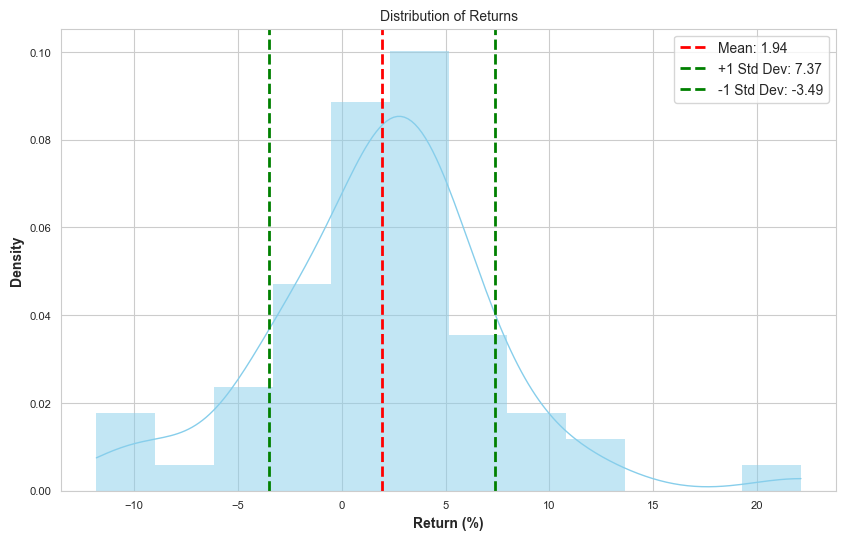
\includegraphics[width=0.7\textwidth]{chapters/Chap4/Monthly_Distribution.png}
    \caption{Distribution of trades with mean returns and standard deviations, showing a generally positive mean return across most months.}
    \label{fig:trade_distribution}
\end{figure}



\thesisspacing
\doublespacing % Do not change - required

\chapter{Conclussion}
\label{ch5}

%%%%%%%%%%%%%%%%%%%%%%%%%%%%%%%%%%%%%%%
% IMPORTANT
\begin{spacing}{1} %THESE FOUR
\minitoc % LINES MUST APPEAR IN
\end{spacing} % EVERY
\thesisspacing % CHAPTER
% COPY THEM IN ANY NEW CHAPTER
%%%%%%%%%%%%%%%%%%%%%%%%%%%%%%%%%%%%%%%

%%%%%%%%%%%%%%%%%%%%%%%%%%%%%%%%%%%%%%%
\thesisspacing % CHAPTER
% COPY THEM IN ANY NEW CHAPTER
%%%%%%%%%%%%%%%%%%%%%%%%%%%%%%%%%%%%%%%

\section{Future Work}

Building on the findings of this study, several directions for future work can be explored to enhance the performance and applicability of the CNN model for financial market prediction. One promising avenue is the integration of more advanced deep learning architectures, such as Transformers, which have recently gained prominence in natural language processing and sequence modeling. Leveraging the advanced computational capabilities of Transformers could potentially improve the model's ability to capture temporal dependencies and complex patterns in financial time series data. This approach may enhance the model's accuracy and robustness, particularly in identifying market anomalies and outlier events.

Another area for improvement involves the use of ensemble methods that combine different model architectures, such as combining time series forecasting models with the existing CNN classifier. This ensemble approach could leverage the strengths of both models, potentially leading to improved predictive performance in both backtesting and forward testing scenarios. Additionally, incorporating more diverse data sources, such as trading volume, macroeconomic indicators, and sentiment analysis from news and social media, could further enrich the feature set available to the model, enabling it to capture a broader range of market signals and conditions. This idea aligns with findings in prior research, such as those by Bryan Kelly, which demonstrated the positive impact of incorporating additional data features on model performance.

Expanding the application of the model to other asset classes, such as currencies, commodities, and bonds, represents another promising direction. Given the model's demonstrated ability to identify significant market moves in U.S. equities, applying it to other markets could provide valuable insights and further validate its robustness and adaptability. Additionally, exploring methods to effectively filter outliers from the dataset prior to training could help reduce overfitting and improve the model’s generalization capabilities.

Finally, enhancing the backtesting framework to include more sophisticated strategies, such as dynamic rebalancing and risk management techniques, could provide a more comprehensive evaluation of the model's real-world applicability. Incorporating forward testing with live market data would also help validate the model's performance under actual trading conditions, further bridging the gap between theoretical research and practical application.

\section{Conclusion}

This study developed and evaluated a Convolutional Neural Network (CNN) model for predicting financial market movements, leveraging time-series data from U.S. stocks. The research demonstrated that CNN models could provide valuable insights into market dynamics and outperform traditional financial forecasting methods under certain conditions. By expanding the dataset beyond the S\&P 500 to include randomly selected U.S. stocks, the model achieved a more comprehensive understanding of diverse market conditions, ultimately leading to a well-performing model with a Sharpe ratio of 1.20 and a drawdown of 24.46\%.

The implementation challenges, particularly around data balancing and overfitting, were addressed through careful data preprocessing and the introduction of regularization techniques such as dropout layers and leaky ReLU activations. The use of a JSON configuration file for model setup allowed for flexible experimentation with different architectures, leading to an optimized model configuration that was effective in backtesting scenarios. The model's ability to identify market outliers, such as the COVID-19 pandemic, further demonstrated its robustness and adaptability.

However, the study also highlighted several limitations, including the tendency to overfit with complex models and challenges in generalizing across multiple asset classes. These findings suggest that while CNNs hold significant promise for financial forecasting, further research is needed to refine these models and explore new architectures and data sources.

In conclusion, this research contributes to the growing body of literature on the application of deep learning techniques to financial markets. The findings underscore the potential of CNNs to enhance predictive accuracy and provide a foundation for more informed investment strategies. Future work focusing on model refinement, the integration of additional data features, and expansion to other asset classes will further enhance the utility and effectiveness of these models in real-world trading environments.



% You can change the title of the conclusions by changing the text between { }
% \conclusions{Conclusions} % Do not remove - required
% EDIT THE CONTENT OF THE FILE
% Conclusions.tex
% You can find it under the folder
% "chapters" on the left column

% APPENDICES ARE OPTIONAL
% COMMENT OUT BOTH LINES BELOW TO REMOVE THEM
% ADD CHAPTERS TO ADD MULTIPLE APPENDICES
\appendix
% \input{AppendixA.tex}
% \input{AppendixB.tex} % Example second appendix (need to create the file in "chapters")


\cleardoublepage % Do not change - required
\RemoveLabels % Do not change - required
\thesisspacing % Do not change - required

\printbibliography[title={Bibliography},heading=bibintoc] % Do not change - required

\end{document}
